%%
%% This is file `sample-sigconf.tex',
%% generated with the docstrip utility.
%%
%% The original source files were:
%%
%% samples.dtx  (with options: `sigconf')
%% 
%% IMPORTANT NOTICE:
%% 
%% For the copyright see the source file.
%% 
%% Any modified versions of this file must be renamed
%% with new filenames distinct from sample-sigconf.tex.
%% 
%% For distribution of the original source see the terms
%% for copying and modification in the file samples.dtx.
%% 
%% This generated file may be distributed as long as the
%% original source files, as listed above, are part of the
%% same distribution. (The sources need not necessarily be
%% in the same archive or directory.)
%%
%% The first command in your LaTeX source must be the \documentclass command.

% drozas: adding this to have subscript without math context
\newcommand\tsub[1]{\textsubscript{#1}}
\newcommand\tsup[1]{\textsuperscript{#1}}


\documentclass[manuscript]{acmart}

%\usepackage{longtable}

%%
%% \BibTeX command to typeset BibTeX logo in the docs
\AtBeginDocument{%
  \providecommand\BibTeX{{%
    \normalfont B\kern-0.5em{\scshape i\kern-0.25em b}\kern-0.8em\TeX}}}

%% Rights management information.  This information is sent to you
%% when you complete the rights form.  These commands have SAMPLE
%% values in them; it is your responsibility as an author to replace
%% the commands and values with those provided to you when you
%% complete the rights form.
%\setcopyright{acmcopyright}
%\copyrightyear{2021}
%\acmYear{2021}
%\acmDOI{10.1145/1122445.1122456}

\setcopyright{rightsretained}

%% These commands are for a PROCEEDINGS abstract or paper.
%\acmConference[OpenSym 2021]{OpenSym 2021: 17th International Symposium on Open Collaboration}{September 15--17, 2021}{Madrid, Spain}
%\acmBooktitle{OpenSym 2021: 17th International Symposium on Open Collaboration,
%  September 15--17, 2021, Madrid, Spain}
%\acmPrice{15.00}
%\acmISBN{978-1-4503-XXXX-X/18/06}


%%
%% Submission ID.
%% Use this when submitting an article to a sponsored event. You'll
%% receive a unique submission ID from the organizers
%% of the event, and this ID should be used as the parameter to this command.
%%\acmSubmissionID{123-A56-BU3}

%%
%% The majority of ACM publications use numbered citations and
%% references.  The command \citestyle{authoryear} switches to the
%% "author year" style.
%%
%% If you are preparing content for an event
%% sponsored by ACM SIGGRAPH, you must use the "author year" style of
%% citations and references.
%% Uncommenting
%% the next command will enable that style.
%%\citestyle{acmauthoryear}

%%
%% end of the preamble, start of the body of the document source.
\begin{document}

%%
%% The "title" command has an optional parameter,
%% allowing the author to define a "short title" to be used in page headers.
%1: \title[The platform belongs to its workers!]{The platform belongs to its workers! Experimenting with worker-centric tools for distribution of value}
%2:\title[The platform belongs to its workers!]{The platform belongs to its workers! Identification of alternative models of distribution of value for worker-centric crowdsourcing platforms}
\title[The platform belongs to those who work on it!]{The platform belongs to those who work on it! Co-designing worker-centric task distribution models}


%%
%% The "author" command and its associated commands are used to define
%% the authors and their affiliations.
%% Of note is the shared affiliation of the first two authors, and the
%% "authornote" and "authornotemark" commands
%% used to denote shared contribution to the research.
%\author{Anonymous Author 1}
\author{David Rozas}
\email{drozas@ucm.es}
\orcid{0000-0001-6371-0964}
\affiliation{
  \institution{Universidad Complutense de Madrid}
  \streetaddress{GRASIA Research Group, Knowledge Technology Institute}
  \city{Madrid}
  \country{Spain}
}

\author{Jorge Saldivar}
\email{jasaldivar@ucm.es}
\affiliation{
  \institution{Universidad Complutense de Madrid}
  \streetaddress{GRASIA Research Group, Knowledge Technology Institute}
  \city{Madrid}
  \country{Spain}
}

\author{Eve Zelickson}
\email{eve@datasociety.net}
\affiliation{
  \institution{Data \& Society}
  \city{New York City}
  \country{United States of America}
}


%%
%% By default, the full list of authors will be used in the page
%% headers. Often, this list is too long, and will overlap
%% other information printed in the page headers. This command allows
%% the author to define a more concise list
%% of authors' names for this purpose.
%TODO: change in final version - anonymised
\renewcommand{\shortauthors}{Rozas, D., Saldivar, J., \& Zelickson, E. (2021)}
%\renewcommand{\shortauthors}{Anonymous Author 1, Anonymous Author 2, \& Anonymous Author 3 (2021)}


%%
%% The abstract is a short summary of the work to be presented in the
%% article.
\begin{abstract}

Today, digital platforms are increasingly mediating our day-to-day work and crowdsourced forms of labour are progressively gaining importance (e.g. Amazon Mechanical Turk, Universal Human Relevance System, TaskRabbit). In many popular cases of crowdsourcing, a volatile, diverse, and globally distributed crowd of workers compete among themselves to find their next paid task. The logic behind the allocation of these tasks typically operates on a ``First-Come, First-Served'' basis. This logic generates a competitive dynamic in which workers are constantly forced to check for new tasks.

This article draws on findings from ongoing collaborative research in which we co-design, with crowdsourcing workers, three alternative models of task allocation beyond ``First-Come, First-Served'', namely (1) round-robin, (2) reputation-based, and (3) content-based. We argue that these models could create fairer and more collaborative forms of crowd labour.

We draw on Amara On Demand, a remuneration-based crowdsourcing platform for video subtitling and translation, as the case study for this research. Using a multi-modal qualitative approach that combines data from 10 months of participant observation, 25 semi-structured interviews, two focus groups, and documentary analysis, we observed and co-designed alternative forms of task allocation in Amara on Demand. The identified models help envision alternatives towards more worker-centric crowdsourcing platforms, understanding that platforms depend on their workers, and thus ultimately they should hold power within them.
\end{abstract}

%%
%% The code below is generated by the tool at http://dl.acm.org/ccs.cfm.
%% Please copy and paste the code instead of the example below.
%%
\begin{CCSXML}
<ccs2012>
   <concept>
       <concept_id>10003120</concept_id>
       <concept_desc>Human-centered computing</concept_desc>
       <concept_significance>100</concept_significance>
       </concept>
   <concept>
       <concept_id>10003120.10003130</concept_id>
       <concept_desc>Human-centered computing~Collaborative and social computing</concept_desc>
       <concept_significance>300</concept_significance>
       </concept>
   <concept>
       <concept_id>10003120.10003130.10011762</concept_id>
       <concept_desc>Human-centered computing~Empirical studies in collaborative and social computing</concept_desc>
       <concept_significance>500</concept_significance>
       </concept>
 </ccs2012>
\end{CCSXML}

\ccsdesc[100]{Human-centered computing}
\ccsdesc[300]{Human-centered computing~Collaborative and social computing}
\ccsdesc[500]{Human-centered computing~Empirical studies in collaborative and social computing}

\copyrightyear{2021}
\acmYear{2021}
\acmConference[OpenSym 2021]{17th International Symposium on Open Collaboration}{September 15--17, 2021}{Online, Spain}
\acmBooktitle{17th International Symposium on Open Collaboration (OpenSym 2021), September 15--17, 2021, Online, Spain}\acmDOI{10.1145/3479986.3479987}
\acmISBN{978-1-4503-8500-8/21/09}

%%
%% Keywords. The author(s) should pick words that accurately describe
%% the work being presented. Separate the keywords with commas.
\keywords{crowdsourcing, digital labour, distribution of value, future of work, human computation, platform economy, task allocation, worker-centric platforms}

%% A "teaser" image appears between the author and affiliation
%% information and the body of the document, and typically spans the
%% page.
%\begin{teaserfigure}
%  \includegraphics[width=\textwidth]{sampleteaser}
%  \caption{Seattle Mariners at Spring Training, 2010.}
%  \Description{Enjoying the baseball game from the third-base
%  seats. Ichiro Suzuki preparing to bat.}
%  \label{fig:teaser}
%\end{teaserfigure}

%%
%% This command processes the author and affiliation and title
%% information and builds the first part of the formatted document.
\maketitle

% !TEX root = 0_main.tex

\section{Introduction}

Contemporary working practices are changing and digital platforms are increasingly mediating our day-to-day work. In this scenario, crowdsourced forms of labour are progressively gaining importance, and large corporations such as Amazon and Microsoft are entering the field. Amazon Mechanical Turk (AMT), Universal Human Relevance System (UHRS), and TaskRabbit are all examples of market-driven crowdsourcing platforms. These platforms operate as labour marketplaces for businesses to outsource work to globally distributed and diverse workers \cite{10.1145/1753846.1753873}. %Upwork is a freelancing marketplace in which customers provide a description of the task and a price range so that freelancers can offer their services. As of 2017 \cite{carrel-billiard_2017}, it had five million registered clients who were annually posting three million jobs to twelve million registered freelancers that were reporting more than US\$1 billion in earnings.

In crowdsourcing platforms, work is ``taskified'' \cite{amer2016toward}. Entering receipts into expense reports, curating data to train an Artificial Intelligence (AI) model, translating texts and tagging words and images, are examples of work that can be easily ``taskified''. These tasks are carried out by an invisible workforce of ``humans in the loop'' \cite{gray2019ghost}. Through platforms such as AMT, in this volatile and globally distributed crowd of workers, with varying degrees of expertise and backgrounds \cite{10.1145/1753846.1753873}, people compete against each other to find tasks to work on. The logic behind the allocation of these tasks typically operates on a ``First-Come, First-Served'' (FCFS) basis \cite{yu2013bringing, han2019all}.

Previous research has argued that FCFS is a convenient method of task allocation because of its simplicity and capacity to decrease task completion time \cite{kamel2020tasks}. The approach, however, creates a competitive dynamic in which workers are forced to be constantly alert for new tasks to appear, producing a sense of anxiety and frustration in case they cannot obtain the work \cite{gray2019ghost}. Additionally, FCFS disadvantages workers who do not have access to a reliable Internet connection or those who work in time zones different from the requesters.
Thus, it can create inequitable work distribution by relying on circumstances that are often beyond workers' control. 

Alternatives of work distribution have been proposed in crowdsourcing literature to optimize worker-task matching, maximising the task-requesters' benefits, and improving results (e.g., \cite{difallah2013pick, ho2012online, karger2014budget, yin2017task}), yet, besides some empirical studies that examine crowdsourcing issues from the workers' perspective (e.g., \cite{mcinnis2016taking, brawley2016work, faullant2013fair}), there is a lack of proposals which aim to improve the working conditions and well-being of workers. This article reports the preliminary results of an interactive design approach where workers have been involved throughout a research process that includes a variety of methods and which aims to identify and validate alternative task allocation logics defined and agreed upon by the workers themselves.

Our vision towards more worker-centric crowdsourcing platforms is summarised by the motto: \textit{``the platform belongs to those who work on it\footnote{We have adapted this motto inspired by Teodoro Flores's phrase ``la tierra es para quien la trabaja'' (``the land belongs to those who work it''), which captures the revolutionaries' vision for land reform in the context of the Mexican Revolution (1910-1920) \cite{mcneely1966origins}.}''}, which aims at empowering workers to define the rules that govern the distribution of value in crowdsourcing platforms.

The remainder of the paper proceeds as follows. Next, we present our case study, followed by a description of the theoretical concepts that frame the work and a review of related works. Section \ref{sec:methods} introduces the methods employed in the study. Later, Section \ref{sec:results} describes the results. A general discussion about the implications of the results is provided in Section \ref{sec:discussion}. We close the paper by presenting conclusions in Section \ref{sec:conclusion}.
% !TEX root = 0_main.tex

\section{Case Study: Amara On Demand}
\label{sec:case-study}

Amara is a project which sustains an open and collaborative platform for the creation of subtitles \cite{jansen_amara_2014}. Examples of organisations employing Amara's platform to create subtitles drawing on volunteer engagement include Khan Academy, Scientific American, and the California Academy of Science \cite{amara}. More specifically, our focus in this research is placed on the use of Amara's platform for the creation of subtitles as an on-demand and paid service: Amara On Demand (AOD). AOD was launched in 2013 \cite{zelickson2019} as a result of the success \cite{jansen_amara_2014} of Amara's platform (Figure \ref{fig:aod-platform} shows a screenshot of AOD's subtitling tool). AOD is organised as a non-profit organisation, under the umbrella of the Participatory Culture Foundation. AOD is inspired by cooperative and commoning practices \cite{gray2019ghost}, presenting a remarkable contrast when compared with the market-based logic of other crowdsourcing platforms. While AOD grew into its own enterprise within \textit{Amara.org}, it adopted the values of the original volunteer community \cite{amaraorg}. %Amara.org’s stated mission captures its commitment to open, collaborative creation that eliminates barriers to accessing online content \cite{amaraorg}.
%\begin{quote}
   % ``We are driven by our mission to foster a media ecosystem that enables everyone to benefit from online video content. Content that can enrich lives, but is not currently available to those who cannot hear or understand the language of the video. We believe a participatory and inclusive world leads to a more understanding and caring society.''
%\end{quote}


\begin{figure}[ht]
    \centering
    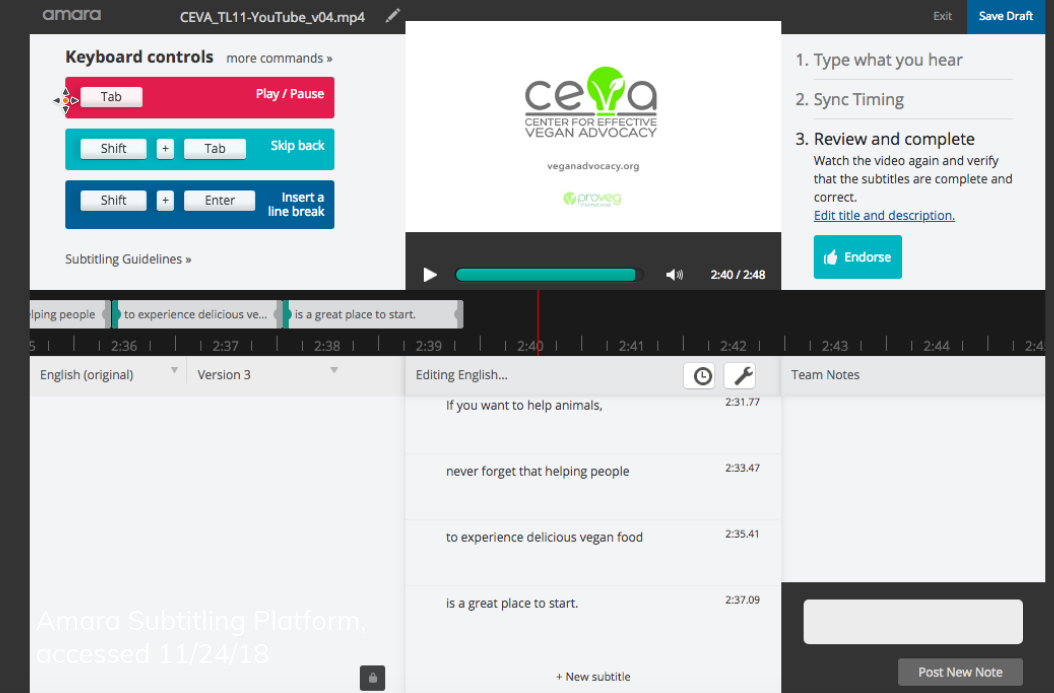
\includegraphics[width=\columnwidth]{figures/AOD_platform.png}
    \caption{Screenshot of AOD's subtitling platform, captured on 24th November 2018.}
    \label{fig:aod-platform}
\end{figure}

Over the past years, AOD moved from a few linguists to more than nine hundred at the time of writing\footnote{As self-reported by key members of AOD's core team during the interviews.} The work of linguists in AOD is remunerated and they are organised on a per-language direction basis and in which English operates as the master language. For example, if a customer requires a set of videos in German to be subtitled into Spanish, this will involve the groups German->English and English->Spanish. In order to join AOD, linguists are required to submit a resume, two examples of captioned or translated work, and pass an online interview as well as a test. The test is intended to ensure linguists understand AOD's guidelines, maintaining quality and thus, client satisfaction.

An essential part of AOD is the core team that facilitates and oversees the whole production process, coordinating and sustaining the infrastructure required for the successful creation of subtitles and captioning. The core team operates as a central node in AOD, although their members are globally distributed. The core team also monitors linguists' compliance with the rules. In AOD, there are explicit rules, practices, and guidelines to govern participation and foster professionalism. For linguists, this means completing tasks by deadlines, not assigning themselves more than one video ``at the same time'', and adhering to project-specific rules. Linguists are expected to adhere to them in order to receive payment.
% !TEX root = 0_main.tex

\section{Theoretical Framework}
\label{sec:theoretical-framework}

Crowdsourcing has many definitions, but can be captured by the idea of an open call for anyone to participate in an online task \cite{brabham2013crowdsourcing, estelles2012towards,howe2008crowdsourcing} by contributing information, knowledge, or skills. The `crowd' refers to the group of people who participate in the crowdsourcing initiative online. The crowd can, in theory, emerge from anyone online or specific subsets of people. Participation is either voluntary (uncompensated) or for money (financially incentivised). An instance of voluntary crowdsourcing can be found in crowdsourced journalism \cite{aitamurto2015motivation} or crowdsourcing in crisis management \cite{schimak2015crowdsourcing}. In paid crowdsourcing, participants are compensated per task, as in microtasking on digital labour market-places such as Amazon Mechanical Turk (AMT) \cite{shank2016using} or based on performance as in innovation challenges \cite{jeppesen2010marginality}.

For this research, we frame our case study as part of the aforementioned broader phenomenon of crowdsourcing. More specifically, we draw on Hansson et al.'s \cite{hansson_capitalizing_2018, hansson_alienation_2017} categorisation of the different modes of production in crowdsourcing platforms to frame AOD as a case of \textit{human computing}.  \textit{Human computing} crowdsourcing platforms, such as Amara and AMT, are those in which ``users do micro-tasks that do not require much expertise, such as transcribing audio and video files, translating texts, or tagging maps [...] [, and in which] individual crowd members usually undertake tasks independently of one another, sometimes even competing for work on this market [...]'' \cite{hansson_capitalizing_2018}. In this study, Hansson et al. \cite{hansson_capitalizing_2018} draw on Marx's \cite{10.2307/2550890} theory of alienation to understand the relationships between participants in crowdsourcing and the role of the platforms employed to mediate in the activities. Marx \cite{10.2307/2550890} described four types of relationships: (1) between producer and consumer, (2) between the producer and product, (3) the producers’ relationship to themselves, and (4) their relationships to other producers. Applying Marx's theory of alienation to crowdsourcing, Hansson et al. \cite{hansson_capitalizing_2018} developed a typology of alienation that reveals significant differences between the cases studied. Figure \ref{fig:hansson_adapted}, adapted from their work, depicts the cases of Amara and AMT. For example, with regards to the relationship between an individual producer with the rest of the producers, the position of Amara being closer towards the inner circle means there are stronger bonds between producers (linguists, in the case of Amara). For the case of AMT, which is in the fourth outer circle, this position represents a lack of bonds between producers. This typology is not to be understood as mutually exclusive: these concepts and different modes sometimes co-exist within the same platforms and processes. However, this typology is ``useful as a way to discuss how participation in crowdsourcing is motivated and to develop tools with a better awareness of different types of relationships and how these modes of productions produce different types of knowledge''.

\begin{figure}[t]
    \centering
    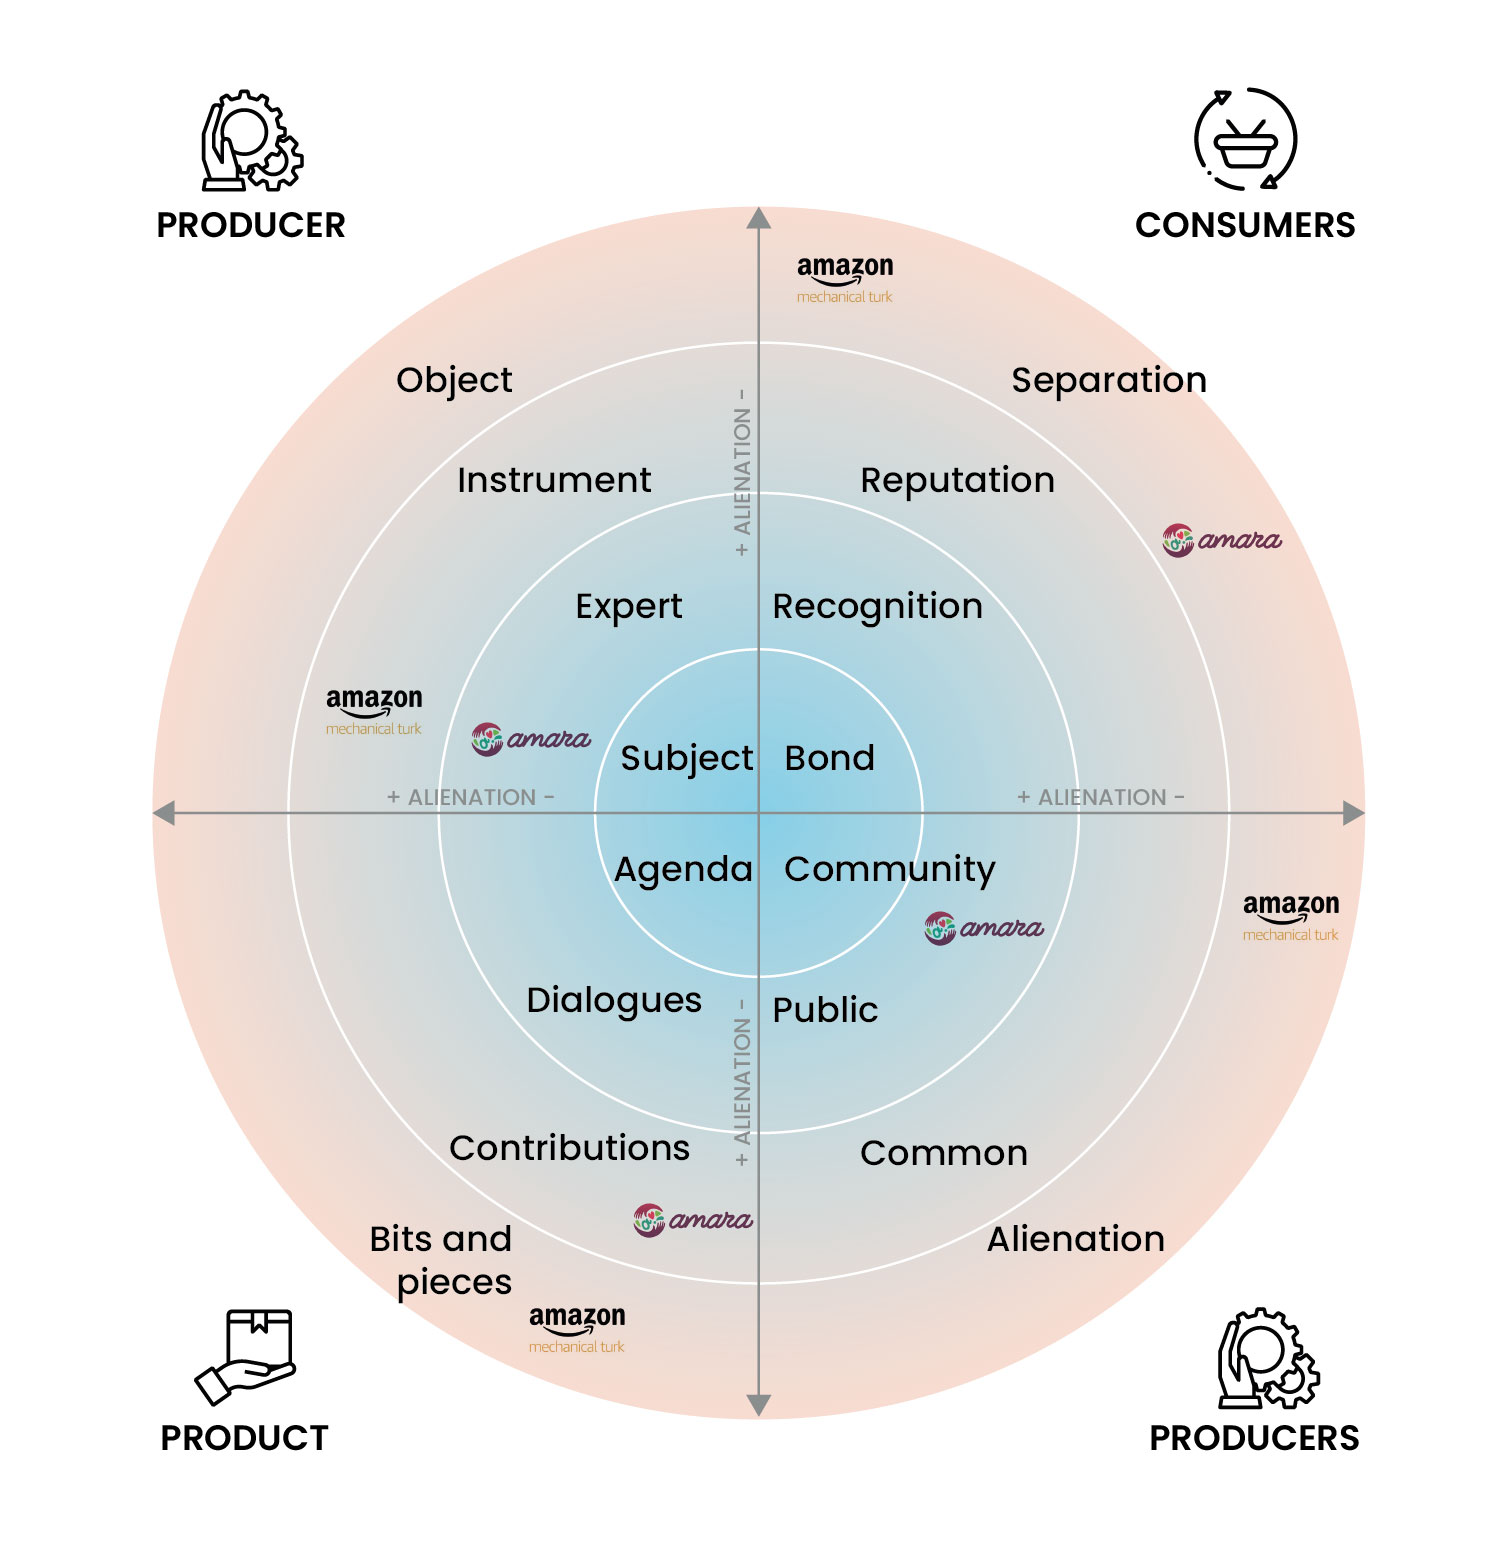
\includegraphics[width=.65\textwidth,height=.5\textheight]{figures/diagrama_02.jpg}
    \caption{A graphic representation of Hansson et al.’s \cite{hansson_capitalizing_2018} typology of alienation, according to Marx’s \cite{10.2307/2550890} four types of relationship. The further from the centre, the higher the degree of alienation. We have adapted Hansson et al.’s \cite{hansson_capitalizing_2018} Figures 1 and 2 in order to merge the categories and the position of the two key cases (from the 21 studied by them) which we employ to establish comparisons: Amara (our case study) and Amazon Mechanical Turk. See Table 4 on \cite{hansson_capitalizing_2018} for further details and a summary of the relationships with corresponding modes of productions and the categories employed.}
    \label{fig:hansson_adapted}
\end{figure}

Drawing on Hansson et al.' typology \cite{hansson_capitalizing_2018} and to further our understanding of how crowdsourcing platforms might support social relationships in these contexts, instead of merely capitalising them \cite{hansson_capitalizing_2018}, we decided to explore the following research question: \textit{can we identify alternative models for the distribution of tasks in crowdsourcing that consider the needs of the workers?}

To this aim, we establish a collaboration with Amara, whose strong cooperative values \cite{gray2019ghost} offer an opportunity to design models of task distribution in which the producer is also the owner of the means of production and the products created are an expression of self-realisation \cite{hansson_capitalizing_2018}. Since, following the concepts from Hansson et al.' typology \cite{hansson_capitalizing_2018} depicted in Figure \ref{fig:hansson_adapted}, Amara contrasts with platforms such as AMT \cite{gray2019ghost}, which understand workers as ``instruments'' from which ``bits and pieces'' can be sourced \cite{hansson_capitalizing_2018}. 


% !TEX root = 0_main.tex

\section{Related Works}\label{sec:related_works}
Various alternatives have been proposed in the literature to allocate crowdsourcing tasks \cite{machado2016task, cui2017complex, mao2015developer, ho2013adaptive, difallah2013pick, kamel2020tasks, zhao2019task, jiang2019group, yu2013bringing, fu2021fairness} as well as to re-think the conditions of crowdsourced labour more generally \cite{kittur2013future,graham2018towards}. Some authors have suggested implementing the power of AI techniques to assign tasks to workers, while other scholars have introduced reputation schemes to delegate tasks. Workers' background, expertise, and social connections have also been considered in approaches presented to improve the assignment of tasks in crowdsourcing platforms.% Others have drawn on distributed computing to re-envisioning crowd work that ``we would want our children to participate in.'' Based on surveying AMT workers, Kittur et al. proposed a new framework for crowd work focused on supporting complex, high-quality work \cite{kittur2013future}. Furthermore, some researchers have envisioned criteria to distinguish fair from exploitative platforms \cite{graham2018towards}.% Along this line, McInnis et al. \cite{mcinnis2016taking} as well as Brawley and Pury \cite{brawley2016work} study the job satisfaction and workers' experiences in crowdsourcing. 

In Machado et al. \cite{machado2016task}, the authors suggest using AI planning to help choose the best delegation strategy based on parameters that configure the crowdsourcing environment, such as task duration and workers' skills. A machine learning-based approach that combines supervised learning with reinforcement learning to infer task allocation strategies that best fit the available rewards and workers' reputation is proposed by Cui and colleagues \cite{cui2017complex}.  A content-based recommendation method is introduced in Mao et al. \cite{mao2015developer} to match crowdsourced development tasks to developers automatically. The system learns from historical activities to favour appropriate workers. Ho et al. \cite{ho2013adaptive} present an algorithm to allocate tasks in situations of heterogeneous tasks or a diverse, skilled workforce.

Difallah and colleagues \cite{difallah2013pick} employ information available in the workers' social network profiles, such as their interests, to automatically assign workers to tasks aligned to them. The matching between workers and tasks is based on a taxonomy derived from categories extracted from workers' interests and descriptions of tasks. Likewise, the construction of workers' profiles using historical data of their performance and data extracted from social networks is suggested in Kamel et al. \cite{kamel2020tasks}. With these data, the authors propose the development of a machine learning model to recommend relevant tasks to workers based on their built profiles. Similarly, Micholia et al., [CITATION NEEDED] developed a framework for task allocation in mobile crowdsourcing marketplaces that relies on identifying users' expertise and interest in performing particular tasks by analyzing their social media profiles. Zhao et al. \cite{zhao2019task} also discuss a model that considers the relationship between workers to assign tasks in crowdsourcing. The proposal is to use social networking sites to learn about the social connections between workers and therefore allocate them and their friends the same or similar tasks.

The allocation of tasks to groups or teams of workers instead of individuals is explored in \cite{jiang2019group}. In group-oriented crowdsourcing, members of naturally existing groups of workers cooperate to perform tasks. Jiang et al. introduce, in this article, the concept of contextual crowdsourcing value, which determines the priority of a group of workers being allocated a task. The contextual crowdsourcing value measures the capacity of the group of workers to complete a given task in coordination with other groups that complement the missing skills of the group's members. Through experimenting with different approaches to gamified crowdsourcing Morschheusera et al. [CITATION NEEDED] found that users preferred crowdsourcing approaches that included cooperation, but found group-based competition to be the most engaging form of crowdsourcing.  

Reputation models for task allocation have been studied by \cite{yu2013bringing}. Here, workers' reputation is estimated based on the workers' past performance, considering the quality of previous work and meeting deadlines. Increasing fairness while reducing costs is proposed by Fu and Liu \cite{fu2021fairness} who introduce a task allocation model (F-Aware) to create fairer crowdsourcing workflows. The proposed approach monitors the execution of workflows, adjusting the operation of the allocation algorithm to achieve a fairer distribution of labour among workers.

Our work contributes a novel perspective of task allocation on crowdsourcing platforms. Instead of proposing an approach that targets cost reduction, budget balance, quality assurance, or timely completion optimisation, as in the reviewed literature, we report on alternative models that have the potential to help allocate tasks in a fairer way drawing on co-designing techniques which allow workers themselves to define task allocation models that improve their welfare in the platform. Previous research has also explored collaborations with workers of the platforms to explore alternatives to change the nature of crowdsourcing work. In response to concerns from AMT workers over a lack of employer accountability, Irani et al. \cite{irani2013turkopticon} developed ``Turkopticon.'' Turkopticon is a platform and browser extension where workers can share experiences about employers, allowing for greater transparency and communication among workers \cite{irani2013turkopticon}. As part of the tool, Turkopticon reveals workers’ views of their task lists with information others have written about employers. AMT workers have also employed generic platforms, such as Reddit, to share advice and experiences of working on AMT \cite{martin2014being, zyskowski2018crowded}. Additionally, researchers in collaboration with AMT workers created a platform called Dynamo to support collective action \cite{salehi2015we}.

However, our study differs from theirs in co-designing directly with AOD workers after establishing a collaboration with the core team that controls and sustains the platform and its code. As discussed in Section \ref{sec:theoretical-framework}, AMT and AOD represent different forms of crowdsourcing platforms, showing us how platforms can increase the alienation of workers, but they can also help to reduce it \cite{hansson_capitalizing_2018}. In this sense, the core team of AOD is willing to experiment with alternative logics that provide more power to the workers themselves and integrate them into the primary platform. In the aforementioned studies \cite{irani2013turkopticon, salehi2015we}, on AMT workers co-designing alternative platforms, the platforms developed represent a form of counter-power, rather than control over the main platform. Next, we provide an overview of the methods employed to follow this co-designing approach.
% !TEX root = 0_main.tex

\section{Methods}\label{sec:methods}

This study employs a multi-modal qualitative approach that combines data collected from 25 online and face-to-face (F2F) semi-structured interviews, ten months of participant observation, focus groups, and documentary analysis of 55 documents, mainly internal AOD documents provided to linguists and official blog posts from \textit{\url{blog.amara.org}}. Table \ref{tab:participants} and Table \ref{tab:participants2} provides an overview of the main characteristics of the participants with whom we conducted semi-structured interviews and organised focus groups. The table includes their gender, main role\footnote{This refers to the main tasks carried out by the participant in AOD. For example, as discussed in Section \ref{sec:case-study} ,whether they are part of the core team. The term DQA refers to Designated Quality Assurer. DQAs are responsible for managing large, active projects where clients often request special instructions. Further details are discussed in Section \ref{subsec:models}.} in AOD, number of years in AOD, location and language groups they belong to (only for linguists), among others. 

%PARTICIPANTS TABLE
%\begin{longtable}{p{.10\textwidth}p{.05\textwidth}p{.15\textwidth}p{.20\textwidth}p{.10\textwidth}p{.05\textwidth}p{.25\textwidth}} 
\begin{table}
\begin{tabular}{lllllll}
\hline
\begin{tabular}[c]{@{}l@{}}Participant\\ID\end{tabular} & Gender & \begin{tabular}[c]{@{}l@{}}Main role\\in AOD\end{tabular} & \begin{tabular}[c]{@{}l@{}}Main translation \\ languages\end{tabular} & \begin{tabular}[c]{@{}l@{}}Country of \\ residence\end{tabular} & \begin{tabular}[c]{@{}l@{}}Years \\ in AOD\end{tabular} & \begin{tabular}[c]{@{}l@{}}Related research \\ method\end{tabular} \\ \hline
%\endhead
P\textsubscript{1} & Male & \begin{tabular}[c]{@{}l@{}}Linguist \end{tabular} & German & Germany & 2 & \begin{tabular}[c]{@{}l@{}}Online semi-structured \\ interview\end{tabular} \\
P\textsubscript{2} & Male & Linguist and DQA & \begin{tabular}[c]{@{}l@{}}Marathi and Hindi \end{tabular} & India & 3 & \begin{tabular}[c]{@{}l@{}}Online semi-structured \\ interview\end{tabular} \\
P\textsubscript{3} & Female & Linguist & Greek & \begin{tabular}[c]{@{}l@{}}United States\\of America\end{tabular} & 7 & \begin{tabular}[c]{@{}l@{}}Online semi-structured \\ interview\end{tabular} \\
P\textsubscript{4} & Female & Linguist & \begin{tabular}[c]{@{}l@{}}Russian and English\end{tabular} & \begin{tabular}[c]{@{}l@{}}United States\\of America\end{tabular} & 3 & \begin{tabular}[c]{@{}l@{}}Online semi-structured \\ interview\end{tabular} \\
P\textsubscript{5} & Male & Linguist and DQA & Greek & Greece & 4 & \begin{tabular}[c]{@{}l@{}}Online semi-structured \\ interview\end{tabular} \\
P\textsubscript{6} & Male & Linguist & Arabic & Egypt & 2 & \begin{tabular}[c]{@{}l@{}}Online semi-structured \\ interview\end{tabular} \\
P\textsubscript{7} & Male & Linguist & \begin{tabular}[c]{@{}l@{}}Dutch and Spanish\end{tabular} & Chile & 6 & \begin{tabular}[c]{@{}l@{}}Online semi-structured \\ interview\end{tabular} \\
P\textsubscript{8} & Female & Linguist and DQA & \begin{tabular}[c]{@{}l@{}}Hindi and English\end{tabular} & India & 2 & \begin{tabular}[c]{@{}l@{}}Online semi-structured \\ interview\end{tabular} \\
P\textsubscript{9} & Female & Linguist & \begin{tabular}[c]{@{}l@{}}Simplified Chinese, \\ Traditional Chinese \\ and Malay\end{tabular} & Malaysia & 2 & \begin{tabular}[c]{@{}l@{}}Online semi-structured \\ interview\end{tabular} \\
P\textsubscript{10} & Female & Linguist and DQA & English & \begin{tabular}[c]{@{}l@{}}United States\\of America\end{tabular} & 5 & \begin{tabular}[c]{@{}l@{}}Online semi-structured \\ interview\end{tabular} \\
P\textsubscript{11} & Female & Linguist & \begin{tabular}[c]{@{}l@{}}French and\\Romanian\end{tabular} & Brazil & 1 & \begin{tabular}[c]{@{}l@{}}Online semi-structured \\ interview\end{tabular} \\
P\textsubscript{12} & Female & Linguist & Greek & Netherlands & 3 & \begin{tabular}[c]{@{}l@{}}Online semi-structured \\ interview\end{tabular} \\
P\textsubscript{13} & Female & Linguist & Russian & Russia & 2 & \begin{tabular}[c]{@{}l@{}}Online semi-structured \\ interview\end{tabular} \\
P\textsubscript{14} & Male & \begin{tabular}[c]{@{}l@{}}Linguist \end{tabular} & \begin{tabular}[c]{@{}l@{}}Portuguese-Portugal\end{tabular} & Portugal & 6 & \begin{tabular}[c]{@{}l@{}}Online semi-structured \\ interview\end{tabular} \\
P\textsubscript{15} & Male & Linguist & Polish & Poland & 2 & \begin{tabular}[c]{@{}l@{}}Online semi-structured \\ interview\end{tabular} \\
P\textsubscript{16} & Male & Linguist & Swedish & Sweden & 4 & \begin{tabular}[c]{@{}l@{}}Online semi-structured \\ interview\end{tabular} \\
P\textsubscript{17} & Female & Accountant (core) & N/A & \begin{tabular}[c]{@{}l@{}}United States\\of America\end{tabular} & 5 & \begin{tabular}[c]{@{}l@{}}F2F semi-structured \\ interview\end{tabular} \\
P\textsubscript{18} & Female & Project Manager (core) & N/A & \begin{tabular}[c]{@{}l@{}}United States\\of America\end{tabular} & 7 & \begin{tabular}[c]{@{}l@{}}F2F semi-structured \\ interview\end{tabular} \\
P\textsubscript{19} & Male & Project Leader (core) & N/A & \begin{tabular}[c]{@{}l@{}}United States\\of America\end{tabular} & 8 & \begin{tabular}[c]{@{}l@{}}F2F semi-structured \\ interview\end{tabular} \\
P\textsubscript{20} & Female & Project Leader (core) & N/A & \begin{tabular}[c]{@{}l@{}}United States\\of America\end{tabular} & 3 & \begin{tabular}[c]{@{}l@{}}F2F semi-structured \\ interview\end{tabular} \\ 
\multicolumn{7}{c}{} \\
\multicolumn{7}{r}{\textbf{Continued on Table \ref{tab:participants2}}} \\ \hline
\end{tabular}
\caption{The participants' main characteristics.}
\label{tab:participants}
\end{table}

\begin{table}
\begin{tabular}{lllllll}
\hline
\begin{tabular}[c]{@{}l@{}}Participant\\ID\end{tabular} & Gender & \begin{tabular}[c]{@{}l@{}}Main role\\in AOD\end{tabular} & \begin{tabular}[c]{@{}l@{}}Main translation \\ languages\end{tabular} & \begin{tabular}[c]{@{}l@{}}Country of \\ residence\end{tabular} & \begin{tabular}[c]{@{}l@{}}Years \\ in AOD\end{tabular} & \begin{tabular}[c]{@{}l@{}}Related research \\ method\end{tabular} \\ \hline
\multicolumn{7}{r}{\textbf{Continued from Table \ref{tab:participants}}} \\
\multicolumn{7}{c}{} \\
P\textsubscript{21} & Non-binary & Developer (core) & N/A & \begin{tabular}[c]{@{}l@{}}United States\\of America\end{tabular} & 2 & \begin{tabular}[c]{@{}l@{}}F2F semi-structured \\ interview\end{tabular} \\ 
P\textsubscript{22} & Female & Project Manager (core) & N/A & Brazil & 6 & \begin{tabular}[c]{@{}l@{}}Online semi-structured \\ interview\end{tabular} \\
P\textsubscript{23} & Non-binary & Recruiter (core) & N/A & \begin{tabular}[c]{@{}l@{}}United States\\of America\end{tabular} & 4 & \begin{tabular}[c]{@{}l@{}}Online semi-structured \\ interview\end{tabular} \\
P\textsubscript{24} & Female & \begin{tabular}[c]{@{}l@{}}Customer service\\(core)\end{tabular} & N/A & Spain & 6 & \begin{tabular}[c]{@{}l@{}}Online semi-structured \\ interview\end{tabular} \\
P\textsubscript{25} & Female & Linguist and DQA & \begin{tabular}[c]{@{}l@{}} Portuguese-Brazilian, \\ English and Spanish\end{tabular} & Spain & 5 & \begin{tabular}[c]{@{}l@{}}F2F semi-structured \\ interview and focus \\ group\end{tabular} \\ 
P\textsubscript{26} & Female & Linguist and DQA & Portuguese-Brazilian & Brazil & 4 & Focus group \\
P\textsubscript{27} & Male & Linguist & Portuguese-Brazilian & Brazil & 7 & Focus group \\
P\textsubscript{28} & Male & Linguist and DQA & Portuguese-Brazilian & Brazil & 5 & Focus group \\
P\textsubscript{29} & Female & Linguist and DQA & Portuguese-Brazilian & Brazil & 3 & Focus group \\
P\textsubscript{30} & Female & Linguist & Portuguese-Brazilian & Brazil & 5 & Focus group \\ \hline
\end{tabular}
\caption{The participants' main characteristics (continuation).}
\label{tab:participants2}
\end{table}
%\end{longtable}

The collected data were coded following an ethnographic content analysis approach \cite{altheide1987reflections}, which involved a continuous process of discovery and comparison of key categories emerging from the data. The various analytical tasks were supported by the Computer‐Assisted Qualitative Data Analysis Software NVivo 12. %Despite the continuous nature, inherent to the taken ethnographic approach, there were two distinctive phases regarding data collection and analysis. 

%TO-KEEP: OLD METHODS TABLE. To keep just in case.

%\begin{table*}[ht]
%\caption{Overview of data collection methods by phases.}
%\label{tab:methods}
%\begin{tabular}{lll}
%\hline
%Method & Phase 1 & Phase 2 \\
%\hline
%Participant observation & \begin{tabular}[c]{@{}l@{}}Field notes created during offline and online \\ participant observation from October 2018 to \\ March 2019\end{tabular} & \begin{tabular}[c]{@{}l@{}}Field notes created during offline and online \\ participant observation from March 2019 to \\ July 2020\end{tabular} \\
%Semi-structured interviews & \begin{tabular}[c]{@{}l@{}}15 semi-structured interviews with linguists from several \\ language groups: Traditional Chinese, Arabic, Greek, \\ Swedish, Portuguese-Brazil, etc.\end{tabular} & \begin{tabular}[c]{@{}l@{}}9 semi-structured interviews with members of \\ the community with a wide range of roles: project \\ managers, developers, co-founders, etc.\end{tabular} \\
%Documentary analysis & 33 internal and public documents & 22 blog posts, mainly from \url{blog.amara.org} \\
%Focus groups & N/A & \begin{tabular}[c]{@{}l@{}}Two-day workshop with several focus group\\sessions with six linguists of the\\ Portuguese-Brazilian team.\end{tabular}\\
%\hline
%\end{tabular}
%\end{table*}

\subsection{Participant observation and interviews} %: October 2018 - March 2019}

%This phase focused on an in-depth analysis of the inner workings of AOD from the perspective of the linguists. 
Online participant observation was carried out over six months (October 2018 - March 2019) to engage with the day-to-day practices of AOD linguists: from the recruitment and onboarding processes to the execution of regular tasks, such as captioning. In addition, 17 semi-structured interviews (see P\textsubscript{1} - P\textsubscript{16} in Table \ref{tab:participants} and P\textsubscript{25} in Table \ref{tab:participants2}) were conducted following a purposive sampling \cite{palys2008purposive} intended to gather the diversity of linguists in terms of language group, experience level, and degree of engagement. The data collected provided us with a rich picture of the experiences, needs and vision of the workflow of an %in participating as an 
AOD linguist. The primary outcomes of this part of the research were the mapping of the workflow of AOD and the identification of an initial set of communitarian needs which led us to discover several intervention points as potential areas to experiment with the development of worker-centric tools to support crowdsourced labour.

A similar approach was conducted but this time with core members of AOD. It involved four months of online participant observation (April 2019 - July 2019), eight semi-structured interviews (see P\textsubscript{17} - P\textsubscript{24} in Table \ref{tab:participants} and Table \ref{tab:participants2}) and documentary analysis of materials generated and posted in the official channels of AOD. As well as with the linguists, the semi-structured interviews were conducted following a purposive sampling \cite{palys2008purposive} with key members of AOD's core team considering the diverse roles in AOD, i.e., project managers, developers, members of the finance team, and project leaders, among others. The data analysis carried out here allowed us to further our understanding of the organisational processes of the workflow and the changes experienced in it over time. The aim was to include all of the different perspectives of the actors involved in the platform, to supplement the information gathered from the linguists. More importantly, the analysis of these data led us to select our point of intervention: task allocation. Task allocation is a necessary precursor to working. As a result, task allocation represents a suitable starting point for envisioning more cooperative labour processes.

\subsection{Focus Groups}

Interviews and participant observations were followed up with an online two-day workshop that included several focus group sessions (organised in June 2020). A call for participation was disseminated through the official AOD channels, including a short survey to show interest in involvement. From all of the linguistic groups in AOD, we chose the Portuguese-Brazilian due to its high degree of organisational complexity. We selected six linguists (see P\textsubscript{25} - P\textsubscript{30} in Table \ref{tab:participants2}) according to their different degrees of experience, since we aimed to have a variety of backgrounds. These focus group sessions allowed us, together with the linguistics, to identify alternative models for allocating tasks. The identified models were subsequently validated by the AOD's core team.

\subsection{Ethical considerations}

The ethical principles described by the European Research Council \cite{erc_ethics} were followed, as well as the recommendations from the Association of Internet Researchers \cite{markham2012}. Drawing on these guidelines, we constantly reassessed so that the discovery of any new issues resulted in remedial action. These actions include anonymising participants and references to customers in field notes and transcripts, in addition to the use of information sheets and consent forms to participate in the interviews and the focus groups.
% !TEX root = 0_main.tex

\section{Results}\label{sec:results}

Next, we describe the series of problems regarding the current logic of task allocation and the main categories surrounding it, which emerged as key from our analysis: (1) first-come, first-served logic, (2) competitiveness, (3) constantly checking for work, and (4) inconsistent workload. Subsequently, we provide an overview of the three alternative models for task allocation identified in this study beyond FCFS.

\subsection{Behind the First-Come, First-Served logic}
\label{subsec:fcfs}

The ``First-Come, First-Served'' logic embedded in the platform is the main component of task allocation in AOD. This logic creates a competitive dynamic between linguists to assign tasks to themselves. The following quote, from an interview with P\textsubscript{4}, depicts the competitive nature associated with FCFS logic:

\begin{quote}
``What I realised very fast is that the competition is absolutely awful, the competition is huge, you need to learn how to get the work.''
\end{quote}

The competitiveness embedded in this logic becomes even more problematic in a global environment, as in the case of AOD. For example, in theory all linguists belonging to the same language group should have the same opportunity to assign themselves a specific task. However, the reality is that some of them might be in time zones that are less convenient concerning the times in which the tasks are usually posted for assignation. Overall, FCFS encompasses a need for workers to check to find more work continuously, an issue identified also in other crowdsourcing projects \cite{gray2019ghost}. For instance,  P\textsubscript{4} explained:

\begin{quote}
``I learnt how to be fast and not sleep with my computer, but [to] wake up with my computer right next to me. There is also a difference in the time zones, [and] I think we are in the worst position. [...] It is competitive even just to grab it [a task]. I need at least 7 hours of sleep. [...] If you really want to get this work, you need to be next to your computer for hours.''
\end{quote}

Furthermore, this FCFS logic needs to be understood in an environment in which the workload is typically inconsistent for most of the language groups, as P\textsubscript{12} explains:

\begin{quote}
``Last year, we only had text work like one month, and the rest of the months we had really short videos, like one minute, two minutes, like an advertisement. So that was it: last year it was poor. But the year before, it was a very, very good year. [...] I would like to make a full wage out of Amara, but I don't have the chance. Maybe later on, if the organisation expands. Because it's cool that you can work from wherever you are, on your own timing.''
\end{quote}

Some linguists also suggested that the competitiveness embedded in the platform's task allocation method undermines the sense of community. P\textsubscript{7}, for example, explained it in the following way:

\begin{quote}
    ``In general, I believe we have a very neutral attitude towards each other because... yes, we share the language. But we are also competing to get the jobs [...]. Especially, in the last couple of years, due to the decline in job orders that I have won, I can tell you that it [competition] is growing.''
\end{quote}

As we introduce in Section \ref{sec:case-study}, one of the key changes implemented by AOD's core was to limit to ``one at a time'' the number of tasks that linguists can assign themselves simultaneously. This change in the logic was a counter-measure to avoid platform vandalism (e.g. it was found that some participants implemented computer scripts to assign themselves tasks as soon as they were published) and as a first attempt to distribute work more equally. Nevertheless, as we have seen, this has not been sufficient to avoid competition between linguists. FCFS is not the most efficient way in terms of productivity either, as the members of the core explained. P\textsubscript{17}, a core member of Amara and one of the key workers responsible for managing the overall organisational processes in AOD, explains the need to increase the throughput and reduce the time provided to linguists to fulfil deadlines:

\begin{quote}
    ``If I'm a linguist, the way it works now is: I'll get a caption [...] whether or not it takes me three days to finish the job, I know in advance it's doable in three days, so I can wait until day three to do it. So I can assign myself on day one and wait until day three and do it. From my perspective and my job [as a manager], I see that as a disadvantage for the company. Because, first of all, the client is going to get it later. [...] also, maybe there was another linguist that could've done it on day one. So, in a way, we do [work `on-demand'] [...], but not in a way in which Uber is on-demand. [...] And we don't have as many people.''
\end{quote}


Considering all of the problems discussed, we organised a co-designing workshop with AOD linguists that allowed us to incorporate their perspectives into the tools that mediate their day-to-day practices. Next, we discuss the three main models which emerged from this initiative.

\subsection{Exploring and identifying alternative models for tasks allocation}
\label{subsec:models}

We identified three alternative models for task allocation beyond FCFS: (1) round-robin, (2) reputation-based, and (3) content-based.

\subsubsection{Round-robin}

Round-robin (RR) refers, in computer science, to an algorithm proposed in the context of operating systems \cite{silberschatz1999applied} to decide how to schedule multiple processes competing simultaneously for CPU time. In RR, computational processes are assigned similar amounts of computing time circularly. It is one of the simplest and most straightforward solutions to avoid \textit{starvation} in-process execution and it is known as one of the fairest scheduling algorithms \cite{tanenbaum2015modern}.

Within the context of the focus group, a parallel with RR emerged when discussing the need to split the work equally between linguists, as P\textsubscript{28} suggested:

\begin{quote}
    ``What I was thinking was a way that all translators could, uh, work on tasks on Amara so that we could split the work equally between translators so that there would be a similar monthly workload for everyone.''
\end{quote}

Rather than in the form of a ``pure RR'', the model was discussed as a starting point that could be customised according to the context to find alternatives in which a more balanced assignation of tasks is achieved. A key aspect related to this model was the ``pre-assignation of tasks'', as depicted by the following excerpt in which participants P\textsubscript{27} and P\textsubscript{28} intervene:

\begin{quote}
    ``P\textsubscript{27}: I was thinking about... about (sic) her idea of pre-assignment. Like, (sic) every day the linguists would come, and we'd have their inbox, uh, the tasks for that day. [...] it could be that on a certain day, uh, we wouldn't have the time needed for that particular task. So it would be necessary to consider, uh, something like the option to accept or not that particular task. [...] 
    
    P\textsubscript{28}: [...] So the translator could be contacted like, uh, they will be given 24 business hours to respond and take a task [...] And the priority would be for someone who's behind this monthly workload. [...]''
\end{quote}

The main advantage discussed by the linguists regarding this model is that it tackles the competitive character discussed in section \ref{subsec:fcfs}, as P\textsubscript{28} explained: 
\begin{quote}
    ``I really liked P\textsubscript{26}'s idea of the pre-assignment of tasks because this takes away the competitiveness aspect of task allocation. [...] This could also be integrated [...] with a spreadsheet that would rank: this translator has worked on this many minutes this month. So the priority would be for a translator who has not worked that many minutes. So that we could, um, reach a fair amount of work for everyone.''
\end{quote}

Indeed, we found that some linguists in Amara already use similar informal practices in their day-to-day operating. While most tasks related to translating and captioning are allocated in AOD following a FCFS logic, reviewing (another type of task) escapes this logic in some cases. This alternative allocation occurs particularly for active projects in which clients often request special instructions. These reviewing tasks are carried out by linguists with more experience and selected by Project Managers. This special role in AOD is known as Designated Quality Assurer (DQA\footnote{As discussed in Section \ref{sec:methods}, DQAs are exclusively responsible for the whole reviewing process for large projects. This contrasts with the usual workflow, in which multiple AOD members review videos within a project following a FCFS logic.}). As the quote by P\textsubscript{28} below depicts, within this specific scope, linguists themselves employ a similar RR logic to balance the workload between themselves:

\begin{quote}
    ``I thought about this because [working as a DQA] I developed a spreadsheet that would sum up all the videos that were available for us to work on, uh, so that we could know which video to allocate to whom like, uh, there's a new video. So if \textit{Emma} was about, I don't know, 20 minutes, uh, shorter than I was, then the video would be given to her. And then the next one would be given to me. And we would find a balance between this workload.''
\end{quote}

As we shall discuss in Section \ref{sec:discussion}, the challenge of this model lies in identifying the specific parameters to encode in these forms of RR allocation and in providing the linguists with mechanisms that enable them to reach consensus among themselves. Furthermore, the parameters of this model could be combined with those from other models, such as the reputation-based system (presented next). Reflecting on these issues, P\textsubscript{27} and P\textsubscript{30} explained:

\begin{quote}
    ``P\textsubscript{27}: [...] there isn’t always a new video to work on. So I think the second part we might have to work on, uh, and I think this could also tie in with my suggestion to split the work equally. So based on the, um, background and the ratings of, uh, translators, they would be pre-assigned to new tasks.[...]  
    
    P\textsubscript{30}: [...] I think attention to deadline is important, and it doesn't matter if you send like a spreadsheet, tell me how many hours, can you work [referring to the calendar idea]. They put like a thousand hours, and then in the day-by-day, you see that they can't, uh, comply to that.''
\end{quote}

Next, we discuss the model of allocation by reputation to which the linguists refer.

\subsubsection{Reputation-based}
\label{subsec:reputation-model}
Reputation systems have been proposed to build trust among Internet users. They are based on collected and aggregated feedback about users' past feedback and help to foster trustworthy behaviours, assess credibility, and discourage dishonest participation \cite{resnick2000reputation}. Usually in crowdsourcing platforms, e-commerce websites, and Q\&A forums, feedback on users' actions is instrumented through textual comments, numerical rating scores such as one-to-five scales, and boolean evaluations (e.g., yes/no, like/dislike) \cite{resnick2006value}. Once built, users' reputation is represented as badges, stars, points, or average scores attached to their screen names \cite{papoutsoglou2020modeling, willems2019reputation, kraut2012building}. 

In the context of AOD, this category emerged as a model in which tasks are offered to linguists according to the quality of their previous work, based on feedback received by their peers, and depending on the characteristics of the tasks themselves. During the workshop, this model emerged as a \textit{points system}. P\textsubscript{27}, for example, proposed the following idea for a model:

\begin{quote}
   ``[...] a system that would be able to rank productivity of linguists [...], something like a points system in which the points would be earned, um, with reference to the volume that was processed before, and also based on the quality of previous work [...]''

\end{quote}

%\begin{quote}
 %  ``[...]a system that would be able to rank productivity of linguists [...], something like a points system in which the points would be earned, um, with reference to the volume that was processed before, and also based on the quality of previous work, [...] and for the sake of transparency, then we could use something like a ranking board where we could see who is doing better, who is who, what needs improvement in the points system [...]''
%\end{quote}

The main problem tackled by this model, according to the linguists, is that it would help to increase the level of transparency within AOD. Currently, in AOD, several levels operate according to the linguist's experience. The transition between these levels, however, currently lacks clarity and explicit mechanisms, as several linguists pointed out. The following excerpt, from an interview with P\textsubscript{2}, illustrates this:

\begin{quote}
    `` [...] About the transition in levels. Translators should know how to reach next levels from the current levels. What's the criteria for that? [...] [we need] transparency on how to move up or just [some] guidelines.''
\end{quote}

Indeed, as with the previous case of informal practices in RR, the transition between the different levels already operates, although it does so without explicit parameters, as P\textsubscript{30} explained:

\begin{quote}
    `` [...] We had knowledge of the previous work that was done by certain linguists that had displayed more quality, more commitment. Uh, they have processed more volume. So [they are promoted] based on all this, but [it was] not, not (sic) quantified, so it was more like a qualitative selection.''
\end{quote}

The challenge of a reputation-based model, as that proposed by the linguists, is arriving at agreements on what to consider within the system. However, within the focus group, linguists found a preliminary consensus regarding its application in the context of the current \textit{AOD levels system}. The system proposed was based on tiers, as the excerpt below by P\textsubscript{28} illustrates:

\begin{quote}
    `` [...] building a tier system based on the [amount of] minutes of videos that translators have worked on. So, um, that could be, for example, three tiers: novice, intermediate, and veteran. So the novice [translators]  would get shorter non-technical videos, and veteran translators would be given the opportunity to work on longer technical videos. And the intermediate [level] would be a balance between the two.[...]''
\end{quote}

The number of possibilities is such that we concluded that specific sessions would be required to fully explore the parameters of this reputation-based model. However, we identified two key characteristics to be incorporated into the design. Firstly, linguists agreed on not only including the final quality of the translation into the system through reviews made by their peers, but the system should also consider if deadlines were met and how well the changes suggested by the reviewer were implemented. The following excerpt by P\textsubscript{30}, illustrates this:

\begin{quote}
   ``[...] I just wanted to add that not only the quality of work should be considered in the scoring system, but also the attention to the deadline. In the past, we had a lot of problems with translators that were good, but they were terrible with deadlines. That actually made us lose some clients.[...]''
\end{quote}

Secondly, the system should promote inclusiveness. For example, linguists expressed their concerns regarding the possible barriers which a reputation-based model could generate. The following quote, from a comment by P\textsubscript{28}, illustrates this concern with regards to the barriers for newcomers:

\begin{quote}
   ``[...] My only worry is that we should be careful not to exclude newcomers. Uh, for example, if, if (sic) a new person received the low rating, uh, we need to ensure this doesn't compromise how much work they get, because this could be, this could turn into a vicious, vicious (sic) circle as the ones who need to practice the most would not be given enough work to improve on. Uh, so  we need to be careful about that. [...]''
\end{quote}

Furthermore, linguists envisioned and proposed ways to tackle such challenges in a reputation-based model. For example, they suggested that linguists' degree of experience should be considered to facilitate the allocation of simpler tasks to newcomers to tackle this type of barrier. Other proposals suggested considering a fixed number of recent tasks carried out:

\begin{quote}
    ``P\textsubscript{30}: [...] So for the newcomers, we should give them shorter videos and simpler subjects. And for the expert translators, the larger videos, longer videos and high profile projects, and high profile clients. [...] 
    
    P\textsubscript{28}: [...] I also thought about rating based on a fixed number of tasks. Like the five or ten latest videos would be taken into account in this rating system, so that upon working on new projects, your ranking could also improve like so that you don't get affected by the first videos. [...]''
\end{quote}

%-----
%TO-KEEP: Perhaps to be used in future versions
%Such system could be combined with the aforementioned characteristics, as PX explained:

%\begin{quote}
   % `` [...] Just reacting to what {Participant 6} was, uh, was saying like, um, the point system could be something like that goes up and down, like, like, (sic) and also like it would be compatible with, with (sic) {Participant 4} idea of, of tiers. Like, like, (sic) um, if you miss a deadline, you lose a point. If you, like, if you promise to take more volume than what you can actually process, you lose a point and then there´s always the risk of going back one tier and then having access to less content. That would be also a motivator.''
%\end{quote}
%-----


In sum, a model based on reputation would help to tackle the need to constantly check for work and increase the degree of transparency of promotions within the platform. However, the model poses a myriad of challenges regarding inclusiveness or the generation of different, and perhaps more challenging, forms of competitiveness. As the previous excerpt illustrates, the model could not be purely based on reputation. It could instead be combined with content-based assignation characteristics, which could help tackle some of these challenges. The next section explores precisely this in our third model: content-based allocation.

\subsubsection{Content-based}
Recommendation systems are the cornerstones of modern online services. In social media, they are used to suggest publications \cite{menk2019recommendation}, in e-commerce sites to offer products \cite{li2015online}, in video-streaming applications to recommend multimedia materials \cite{davidson2010youtube}, and in crowdsourcing platforms to suggest tasks to workers, as we saw in Section \ref{sec:related_works}. Content-based is one of the most widely used techniques employed in recommendation systems. It focuses on matching the characteristics of the artefact to recommend (e.g., topic of publication, movie genre or task description) with attributes of users based on their profiles and historical data \cite{isinkaye2015recommendation}. 

For our case study, this model emerged as one in which tasks are pre-assigned according to two different types of possible matching logics: (1) either the linguist's skills and/or personal preferences regarding specific areas of knowledge, and (2) the linguist's previous experience in the platform concerning the complexity and/or size of the task.

The former initially emerged from discussions on how to ensure the quality of translations, as the following excerpt by P\textsubscript{26} depicts:
\begin{quote}
    ``[...] if people work based on their backgrounds, they're much more used to [the] terminology and that, in the end, increases the quality.''
    %in the, in the end. I think that´s a pretty good idea. And, but yeah, this, if I think about, uh, Amara’s, no? The way the Amara works and so how this could be done, no. So how the, how this work could be allocated because besides technical work there is, we do a lot of, uh, not a lot, but some movies and other things, no. So how this other work that´s not technical in the specifics would be allocated also is something I think we would have to think about it in the end, but I don´t know why.
\end{quote}

The initial ideas revolved around attempts to match the linguist's skills to the content of the video to be subtitled. For example, some of the participants in the focus group possessed a degree in Law. Therefore, some argued that the model should prioritise them to complete tasks involving videos concerning Law. This proposal, however, did not reach a consensus. As other linguists argued, sometimes they prefer to work on contents that are not part of their official background:

\begin{quote}
     ``P\textsubscript{27}: [...] not working only on what we are already specialised in, but having the chance to learn something new. Sometimes that's  even the main motivation: entering a new field, uh, learning a new subject, dealing with a completely different area, different worlds. Like we come from from (sic) Law. And we are working as linguists precisely because we didn't like Law that much (laugh).
     
     P\textsubscript{30}: [...] I think not only [the] backgrounds of the translators should be considered, but also [their] interests. You know, people have hobbies, people like some sort of movies and [some] kinds of stuff more than others. So I think we should also be considering not only like, you know, university backgrounds, but also personal interests.''
\end{quote}
 
As with the case of the reputation-based models discussed in subsection \ref{subsec:reputation-model}, we concluded specific focus groups would be required in order to explore the details of this model. Nevertheless, an initial consensus emerged about considering the contents of previous tasks as a possible avenue to explore and implement this type of model:

\begin{quote}
     ``P\textsubscript{27}: [...] we could define this background and this specialisation of interests based on the most recent work [...] their most recent work in the previous weeks or the previous months [...]
     
     P\textsubscript{25}: [...] maybe considering also the size [...] like the five last big videos that the person has worked with would define their, (sic) their interests or their, (sic) [areas of] specialisation.''
\end{quote}

The session concluded by discussing logics which could, therefore, be potentially merged with those from reputation-based models, in which the complexity and the size of the task would also be considered when carrying out this content-based assignation, as the excerpt below including an intervention by P\textsubscript{26} depicts:

\begin{quote}
    ``[...] I think that may be one way to do that. Eh, like new people would get more priority on smaller jobs, and then people with more experience get priority with larger jobs. And then people, as they get experience, they start working on longer videos. [...] we know that if a person has had little experience before, then [it] is a bit complicated. So maybe the way would be prioritising smaller videos to newcomers, so everybody would have a chance to improve and to learn.''
\end{quote}

As with the previous cases, content-based models have the potential to be helpful in overcoming some of the problems for workers derived from the predominant FCFS logic, as those described in Section \ref{subsec:fcfs}. The three identified models presented in this section are, however, to be understood as ideal types \cite{weber1904objektivitat}. These models are not necessarily a description of reality as such, but valuable concepts when employed as methodological tools to systematise and consider facts that enable us to analyse and intervene within this specific social context. Therefore, identifying these models provides us with a helpful starting point to structure and guide our research, enabling the possibility of establishing comparisons between them and identifying specific characteristics that facilitate merging features of one model with the characteristics of another. Next, we discuss our results concerning the previous literature in the area and provide an overview of future avenues for research with the models mentioned above.
% !TEX root = 0_main.tex

\section{Discussion}
\label{sec:discussion}

Conceptualising more egalitarian working conditions in crowdsourcing in collaboration with workers is not unique to this study \cite{kittur2013future,graham2018towards}. Nevertheless, our focus on alternate forms of task allocation \textit{within} a cooperative crowdsourcing organisation — as opposed to platforms like AMT — is. Most large crowdsourcing platforms are less cooperative than AOD, making it challenging to alter aspects of the platform. This study illustrates the potential of co-designing hand-in-hand with workers and the significance of task allocation in dictating the nature of work. % Nevertheless, there remains a lack of research exploring how to engage workers in re-imagining a more transparent and equal process for obtaining work.% Projects such as The Drivers Cooperative, a worker-run ride-hailing cooperative in New York City, are heading in this direction.

Previous research has criticised algorithmic task allocation — typical in ridesharing platforms like Uber and Lyft — for its opacity and control over workers' profiles, routes, customers, and wages. As reported by Gray and Suri in \cite{gray2019ghost}, and confirmed in this research, current task allocation methods used in crowdsourcing platforms, which are primarily governed by an FCFS logic, generate competitive dynamics that result in an unfair and unequal distribution of labour and a sense of frustration among workers. We also found that the inherent competitiveness imposed by FCFS also harms the relationship between workers, negatively impacting the sense of community.

Our research in collaboration with AOD's workers allowed us to define alternative methods to FCFS for task allocation. Through a multi-modal methodology that included interviews, participant observation, focus groups and documentary analysis, we identified together with AOD's workers three models that could allocate tasks considering their needs.

The review of the literature demonstrates that most task allocation approaches are focused on optimising the needs of task requesters. These task-requester-centric solutions are intended to reduce costs \cite{ho2012online}, maximise matching \cite{machado2016task}, and increase the quality of results \cite{yu2013bringing}. Fairness in task allocation has been discussed by Fu and Liu \cite{fu2021fairness}. However, their solution focuses on creating fair crowdsourcing workflows, i.e., a logically related series of tasks, by minimising costs. In contrast, our work aims to shift the current FCFS logic of task allocation for models designed by workers to create cooperative and more equitable working conditions.

In this sense, round-robin (RR), one of the identified models, was proposed by the participants to create a more balanced workload. In RR, tasks are pre-assigned to workers in rounds, reducing the competitive dynamics of the current FCFS allocation practice. Although there was consensus among  participants that having a model that pre-assigns tasks in rounds could improve their experience in the platform, there are still essential implementation details in question. In the forthcoming focus groups with linguists, we will examine the rules and parameters that will define the operation of the model. For example, how does the availability of workers impact the model? How does the complexity of tasks affect the assignation of labour? How does worker expertise influence the distribution of tasks?

In discussing workers' expertise, the participants expressed that a reputation-based model might be a valuable complement to RR. In this context, workers' reputation would be captured through a system that reflects workers' performance based on historical feedback. Although performance-based reputation systems are already part of crowdsourcing platforms (e.g., Waze, TaskRabbit, AMT), participants see this model as applicable to improve transparency in the promotion mechanisms used in AOD. Here, workers need to build a ``career path'' by moving through different stages to reach higher levels of responsibility within the organisation. The significant concern with the reputation model, according to participants, is discrimination against newcomers and low-rated workers as well as task concentration by highly-rated workers. Brawley and Pruy have also mentioned the harmful impacts of reputation systems in crowdsourcing platforms in \cite{brawley2016work}. The participants suggest distributing more straightforward tasks to novices to promote inclusiveness, ensuring that they have assigned tasks when joining the platform.
As with the case of RR, there are implementation details to be addressed, and we plan to organise specific focus groups with linguists to explore them. It is still unclear, for example, what aspects of workers' history should be factored into one's reputation. Apart from workers' level and their historical performance, some participants suggested other elements such as attention to past deadlines, caring work \cite{10.3389/fhumd.2021.618207} (e.g., welcoming and tutoring newcomers), and consideration of colleagues' feedback. Gamification techniques based on artefacts that represent participants' reputation (e.g., badges, points, ranking) \cite{feng2018gamification} were also discussed as potential features to equip reputation-based models. 

A task allocation model that includes features of the tasks (e.g., complexity, size, topic, length) and workers' skills, background, and preferences was also seen by the participants as a suitable complement to reputation systems. Apart from complementing the reputation model, this method has been found advantageous to match workers with their expertise and skills resulting in high-quality tasks. Alternatively, some participants indicated that assigning tasks that are not necessarily related to workers' abilities and background might favour learning opportunities for workers. The parametrisation of this content-based model was also left for the next round of focus groups with the participants. It remains unclear how workers' domain of expertise should be included in the model and how to operationalise workers' preferences and interests.

The results presented in this article cannot, however, be generalised and should be understood within the particular case of AOD and similar crowdsourcing platforms. Moreover, due to our qualitative approach, the results cannot be generalised within AOD, considering other groups of linguists may relay a significantly different context, and therefore other models might be more suitable for them. In order to tackle this, we are currently carrying out a longitudinal quantitative analysis of the relationship between users and their activities, drawing on the data already available on AOD’s platform. Drawing on this data, we plan to carry out a similar research process with linguists of other language groups (e.g., English-Japanese, English-Italian, English-Spanish).

Furthermore, we want to explore how to develop tools which allow crowdsourcing workers to decide on the models to use in different contexts. Similarly, these tools to support decision-making could be employed to determine collectively how a model could be parameterised. In doing so, we plan to  develop collaborative decision-making tools that leverage the affordances \cite{doi:10.1177/21582440211002526, 10.3389/fbloc.2021.577680} of distributed-ledger technologies, such as blockchains, to allow crowdsourcing workers to prioritise parameters within the models which better suit their needs, as well as to decide collectively between the models themselves. In the context of our case study, a blockchain-based solution might enable linguists belonging to different language groups to self-organise in Decentralised Autonomous Organizations (DAOs) and resolve task allocation mechanisms that satisfy their requirements\footnote{See \cite{el2020overview} for an overview of how organisations have been using blockchain technologies with the aim to decentralise governance.}. Given that the results are part of a work-in-progress research endeavour, whether the identified models help to reduce competitiveness and improve  working conditions is to be validated.

% !TEX root = 0_main.tex

\section{Conclusion}\label{sec:conclusion}
This article reports on an endeavour to engage crowdsourcing workers in a multi-modal user-centred research process to identify alternative models of value distribution in crowdsourcing platforms. Three models have emerged as a result of the process, namely (i) round-robin, (ii) content-based, and (iii) reputation-based. Although the proposed models have the potential to improve the workers' experience in crowdsourcing platforms by distributing tasks more fairly, implementation details need to be discussed in subsequent research. Our aim is for this line of research to impact beyond this case study to broader areas of the platform economy. Ultimately, our goal is to foster workers' participation in and ownership of the platforms that mediate their work. Similar platforms owned by cooperatives of workers, distributing tasks and value according to the agreements reached by them, could be envisioned for a variety of areas. An example could be a cooperative of taxi drivers whose organisation is mediated by a platform which they control. The platform could distribute and monitor rides and payments according to the rules defined by the workers within their specific context.

 In sum, despite the inherent limitations due to the ongoing nature of this research, the models identified throughout the collaboration with AOD show us that it is possible to envision more cooperative models to distribute work, in which the producers progressively become owners of the means of production and the fruits of their labour expressions of self-realisation \cite{hansson_capitalizing_2018} and, as a result, \textit{platforms might belong to those who work on them}.

%%
%% The acknowledgments section is defined using the "acks" environment
%% (and NOT an unnumbered section). This ensures the proper
%% identification of the section in the article metadata, and the
%% consistent spelling of the heading.
\begin{acks}
This work was partially supported by the project P2P Models (https://p2pmodels.eu) funded by the European Research Council ERC-2017-STG (grant no.: 759207) and by the project Chain Community funded by the Spanish Ministry of Science, Innovation and Universities (grant no.: RTI2018-096820-A-100). We thank all the members of the AOD community: their help made this research possible. A special mention goes to all the linguists who participated in the focus group and the interviews. We also thank the anonymous reviewers for their suggestions. We are also grateful to all of our friends and colleagues of P2PModels for their helpful comments, guidance and advice. We are particularly thankful to Elena Martínez-Vicente and Paulo Colombo for their help organising the focus group and their overall work in the case study. Finally, we would like to thank Tabitha Whittall for her help in copyediting and proofreading this article.
\end{acks}

%%
%% The next two lines define the bibliography style to be used, and
%% the bibliography file.
\bibliographystyle{ACM-Reference-Format}
\bibliography{bibliography}

%%
%% If your work has an appendix, this is the place to put it.
%\appendix

\end{document}
\endinput
%%
%% End of file `sample-sigconf.tex'.
